\section{Part 5}
Example 8.11 was simulated to plot the power curve for one sample \textit{t} testing. Figure \ref{fig:part5} was reproduced below with the following snippet:

\begin{lstlisting}
    sigma <- 0.1  # standard deviation
    alpha <- qnorm(1-0.05)  # P(Z > alpha)
    xSeq <- c(0, 0.2)  # x bounds

    png(
        filename="figures/part5.png", 
        units="in", width=6, height=4, res=200
    )
    ggplot(NULL, aes(x=x, colour=n, fill=n)) +
        stat_function(data=data.frame(x=xSeq, n=factor(5)), 
            fun=function(x) { pnorm(sqrt(5)*x/sigma - alpha) }) +
        stat_function(data=data.frame(x=xSeq, n=factor(10)), 
            fun=function(x) { pnorm(sqrt(10)*x/sigma - alpha) }) +
        stat_function(data=data.frame(x=xSeq, n=factor(15)), 
            fun=function(x) { pnorm(sqrt(15)*x/sigma - alpha) }) + 
        ylab("Power") + xlab("Difference") + labs(colour="Sample Size")
    dev.off()
\end{lstlisting}


    \begin{figure}[ht]
        \begin{center}
            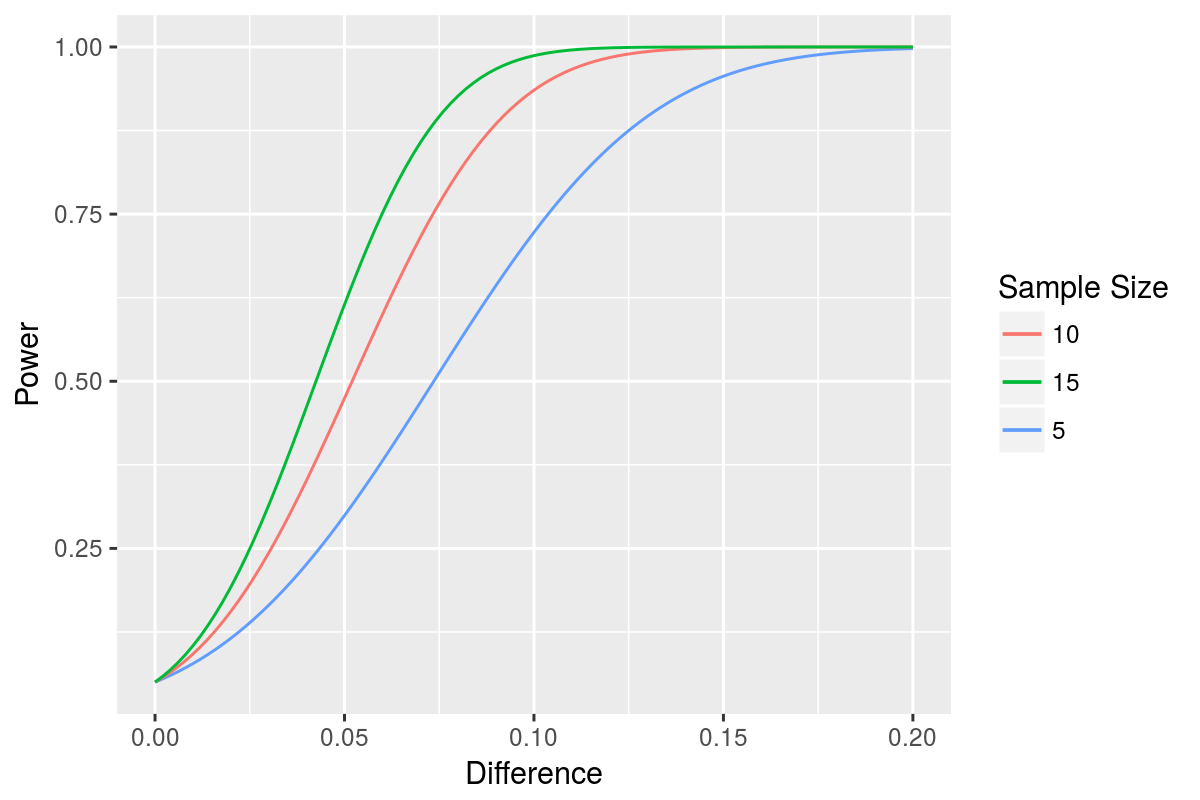
\includegraphics[width=0.7\textwidth]{figures/part5.png}
            \caption{Power Curves for the \textit{t} test Simulated from Example 8.11} \label{fig:part5}
        \end{center}
    \end{figure}
